% CVPR 2026 Paper Template; see https://github.com/cvpr-org/author-kit

\documentclass[10pt,twocolumn,letterpaper]{article}

%%%%%%%%% PAPER TYPE  - PLEASE UPDATE FOR FINAL VERSION
 \usepackage{cvpr}              % To produce the CAMERA-READY version
%\usepackage[review]{cvpr}      % To produce the REVIEW version
% \usepackage[pagenumbers]{cvpr} % To force page numbers, e.g. for an arXiv version

% Import additional packages in the preamble file, before hyperref
\input{preamble}

% It is strongly recommended to use hyperref, especially for the review version.
% hyperref with option pagebackref eases the reviewers' job.
% Please disable hyperref *only* if you encounter grave issues, 
% e.g. with the file validation for the camera-ready version.
%
% If you comment hyperref and then uncomment it, you should delete *.aux before re-running LaTeX.
% (Or just hit 'q' on the first LaTeX run, let it finish, and you should be clear).
\definecolor{cvprblue}{rgb}{0.21,0.49,0.74}
\usepackage[pagebackref,breaklinks,colorlinks,allcolors=cvprblue]{hyperref}

%%%%%%%%% PAPER ID  - PLEASE UPDATE
\def\paperID{25} % *** Enter the Paper ID here
\def\confName{CVPR}
\def\confYear{2026}

%%%%%%%%% TITLE - PLEASE UPDATE
\title{Comprehensive Road Scene Understanding for Autonomous Driving: \\ Semantic Segmentation to Anomaly Detection with EoMT}

%%%%%%%%% AUTHORS - PLEASE UPDATE
\author{
Omer Ozkan \quad Ceylin Afyoncu \quad Franck Hernold Kewo Kameni \\
Politecnico di Torino \\
Student IDs: s360761, s346382, s359890 \\
{\tt\small \{s360761, s346382, s359890\}@studenti.polito.it}
}

\begin{document}
\maketitle
\begin{abstract}

Semantic and anomaly segmentation are critical for autonomous driving. 
But predefined-class models fail on the unknown objects, and it creates danger in the real world scenarios. 
We evaluate EoMT (encoder-only mask transformer with DINOv2 backbone) on semantic segmentation, and we compare COCO-trained EoMT (55.17\% mIoU) with Cityscapes-trained EoMT (81.68\% mIoU) on Cityscapes validation dataset. 
We fine-tune the COCO-EoMT on Cityscapes which reaches to 78.85\% mIoU. 
For anomaly segmentation, we compare ERFNet and EoMT models using four post-hoc scoring methods which are MSP, MaxLogit, MaxEntropy, and RbA on 5 different datasets. 
Our findings show that EoMT-Cityscapes with MSP reaches 74.36\% AuPRC on RoadAnomaly21. 
Our code is available at \url{https://github.com/omerzkan/eomt-anomaly-segmentation}.

\end{abstract}

    
\section{Introduction}
\label{sec:intro}

Semantic segmentation analyzes every pixel and classifies each one into related class. 
A vehicle needs to know where pedestrians are and where the road is. Without pixel-level analysis, this task is difficult. 
The Cityscapes dataset~\cite{cityscapes} is a standard benchmark for this type of task. It includes 5000 photos of German streets. 
Each photo is manually labeled with 19 classes such as road, sidewalk, building.
ERFNet~\cite{erfnet} is a traditional pixel-based approach. 
It uses a CNN (convolutional neural network) with an encoder-decoder architecture, and classifies each pixel independently.
MaskFormer~\cite{maskformer} changed this approach by predicting N binary masks and N class labels, then combining them. 
In this way, the model handles both semantic and panoptic segmentation~\cite{panoptic}. 
Mask2Former~\cite{mask2former} improved MaskFormer by adding masked cross-attention, so the model only looks at the image region where each mask is predicted. 
EoMT~\cite{eomt} simplified this further. It uses only the DINOv2~\cite{dinov2} encoder and removes the pixel decoder entirely.
The problem is that all these models are closed-set. 
They were trained on exactly 19 classes, and during training they did not see anything except what were trained on. 
However, the model must assign objects it has never seen to one of its known classes. 
if the model assigns an animal or fence as road, the vehicle tries to drive through it. This creates safety problems. 
This type of data is called out-of-distribution (OoD) data. 
We use four post-hoc scoring methods (MSP, MaxLogit~\cite{maxlogit}, MaxEntropy~\cite{maxentropy}, RbA~\cite{rba}) with temperature scaling, and evaluate them on benchmarks from SMIYC~\cite{smiyc} and Fishyscapes~\cite{fishyscapes}.
We evaluated EoMT on semantic segmentation and compared two differently trained models (COCO-EoMT vs Cityscapes-EoMT).
Then we fine-tuned the COCO-EoMT on Cityscapes, and the model achieved 78.85\% mIoU. 

\section{Methodology}
\label{sec:method}

\subsection{Semantic Segmentation}

Semantic segmentation was our first task, and we used EoMT~\cite{eomt}, which is a mask-based architecture built on a DINOv2-pretrained Vision Transformer~\cite{dinov2}. Mask classification predicts a fixed set of $K$ masks with a class label for each mask. This idea was introduced by MaskFormer~\cite{maskformer} and improved by Mask2Former~\cite{mask2former}. EoMT removes the convolutional adapter and the pixel decoder, simplifying the mask-based pipeline. It only uses the pretrained ViT to extract features.

We compared two EoMT models using two different checkpoints: EoMT-COCO and EoMT-Cityscapes. A checkpoint contains the model weights learned from a specific dataset, so the same architecture behaves differently depending on which checkpoint is loaded. EoMT-COCO is trained on the COCO dataset, a large general-purpose dataset with 118k training images covering daily scenes such as streets, kitchens, beaches, and animals. COCO has 133 class labels: 80 ``thing'' classes such as person, car, and dog, and 53 ``stuff'' classes such as sky, grass, wall, and sand. This makes the model strong on a wide range of visual objects, but it is not road-specific.

The second model is EoMT-Cityscapes, trained on the Cityscapes dataset. Cityscapes is a smaller dataset (around 3k training images) of road and driving scenes from German cities. It has 19 class labels specifically chosen for autonomous driving, such as road, sidewalk, building, pole, traffic light, traffic sign, person, rider, car, and bicycle. It is road-specific but not as broad as COCO.

We evaluated both models on the Cityscapes validation set, which contains 500 images. The goal was to understand how much a general model loses compared to a specialized one, and whether fine-tuning can close the gap. To do this, we had to solve one problem: EoMT-Cityscapes has 19 output channels matching the 19 Cityscapes classes, while EoMT-COCO has 133 output channels matching the 133 COCO classes. We had to translate the COCO predictions into the Cityscapes label space before evaluation.

We built a \texttt{coco\_to\_cityscapes.py} mapping that works in three steps:
\begin{itemize}
    \item \textbf{Direct name match:} obvious matches found by string comparison. For example, COCO ``car'' maps directly to Cityscapes ``car'', and COCO ``person'' to Cityscapes ``person''.
    \item \textbf{Synonyms:} some classes are named differently in the two datasets. We built a synonym dictionary to handle these cases. For example, COCO calls sidewalks ``pavement-merged''.
    \item \textbf{Ignored:} COCO labels with no Cityscapes equivalent are mapped to the ignore index 255, which excludes them from evaluation. For example, if EoMT-COCO predicts ``dog'', that pixel is ignored.
\end{itemize}



For each of the 19 Cityscapes classes we compute the Intersection-over-Union (IoU):
\begin{equation}
\mathrm{IoU}_{c} = \frac{TP_{c}}{TP_{c} + FP_{c} + FN_{c}}
\label{eq:iou}
\end{equation}
The mean IoU (mIoU) is the average over the 19 classes. It treats every class equally, so rare classes count as much as common ones.

\subsection{Fine-Tuning}
In fine-tuning, we take a model which is already trained on a dataset and continue training on a 
new dataset while keeping the useful information from previous trainings. 
We chose fine-tuning because EoMT-COCO is broad and powerful, but not road-specific. 
We wanted to see if we could adapt it to the Cityscapes domain without losing its general knowledge.

When fine-tuning EoMT-COCO, we dropped the classification head because COCO's classification 
head produces 133 logits per query, one per COCO class. We replaced it with a new head that has 19 outputs which is one per Cityscapes class.
The rest of the weights are kept from the EoMT-COCO. 
For efficiency, we froze the DINOv2 backbone and trained only the queries, mask module, and the new classification head. 
We also use Automatic Mixed Precision (AMP). Instead of FP32, we use mixed-precision FP16.
For the training setup we used $20$ epochs, $K=200$ queries, image size $640{\times}640$. 
Training was done on a single NVIDIA L4 GPU via Google Colab Pro.
For the loss function we used standard Mask2Former~\cite{mask2former} loss.
It combines Hungarian matching between predicted and ground-truth masks, with cross-entropy on classes and Dice + binary cross-entropy on masks.
We use AdamW with a learning rate of $1\times10^{-4}$.

\subsection{Anomaly Segmentation}
We evaluate ERFNet and EoMT under anomaly segmentation.
Anomaly segmentation detects pixels belonging to objects which are not found in the training class set. We can say that these pixels are out-of-distribution.
For evaluation, we use post-hoc methods which use model's class logits, do not require retraining, and calculate anomaly score per pixel. 
Both ERFNet (pixel-based) and EoMT (mask-based) produce class logits, and this allows us to use the same scoring functions for both models.
For evaluating the models, we consider four scoring methods.
\paragraph{Post-hoc anomaly detection methods.}
\begin{itemize}
    \item \textbf{MSP (Maximum Softmax Probability):} uses the highest softmax probability as an uncertainty indicator.
    \begin{equation}
    \text{score}_{\text{MSP}}(\mathbf{x}) = 1 - \max_c p_c(\mathbf{x})
    \end{equation}
    
    \item \textbf{MaxLogit:} uses the raw logits before softmax, because they preserve the magnitude of the model's confidence.
    \begin{equation}
    \text{score}_{\text{MaxLogit}}(\mathbf{x}) = -\max_c L_c(\mathbf{x})
    \end{equation}
    
    \item \textbf{MaxEntropy:} if the probability is spread across many classes (high entropy), the model is uncertain and the pixel is a possible anomaly. If it puts all probability on one class (low entropy), the model is confident.
    \begin{equation}
    \text{score}_{\text{Entropy}}(\mathbf{x}) = -\sum_{c=1}^{C} p_c(\mathbf{x}) \log p_c(\mathbf{x})
    \end{equation}
    
    \item \textbf{RbA (Reweighted by Area)~\cite{rba}:} only for mask-based models. It does not work with ERFNet~\cite{erfnet}. 
    RbA flags pixels that are not strongly claimed by any mask. RbA relies on an independence assumption: in a mask architecture, 
    each class behaves like a one-vs-all classifier, so class probabilities do not need to sum to 1.
    In a pixel-wise classifier like ERFNet, the class probabilities must sum to 1.
    The independence assumption is violated, and RbA doesn't have the same OoD-detection meaning. That's why we don't apply RbA to ERFNet.
    \begin{equation}
    \text{score}_{\text{RbA}}(\mathbf{x}) = -\sum_{c=1}^{C} \tanh(L_c(\mathbf{x}))
    \end{equation}
\end{itemize}


\paragraph{Temperature scaling.}

It is a calibration technique that can shift recall and precision in anomaly detection.
It divides logits by $T$ before softmax. $T > 1$ makes probabilities more uncertain, $T < 1$ makes them more confident. 
We tested $T \in \{0.5, 0.75, 1.0, 1.1, 1.5, 2.0\}$ on MSP, MaxEntropy, and RbA. We didn't test on MaxLogit, which doesn't use softmax.

\paragraph{Datasets and metrics.}

As evaluation benchmarks, we use a smaller subsets of these five datasets which are provided by course instructors. These are:

\begin{itemize}
    
    \item \textbf{RoadAnomaly21 (from SMIYC~\cite{smiyc}):} 10 images, large unknown objects in diverse environments.
    \item \textbf{RoadObstacle21 (from SMIYC~\cite{smiyc}):} 30 images, small unknown objects on the road.
    \item \textbf{Fishyscapes Lost\&Found~\cite{fishyscapes}:} 100 validation images of real lost-cargo objects.
    \item \textbf{Fishyscapes Static~\cite{fishyscapes}:} 30 images, synthetic anomalies on the road scenes.
    \item \textbf{RoadAnomaly (from SMIYC~\cite{smiyc}):} 60 images, earlier version of SMIYC's anomaly track.     

\end{itemize}
We use two metrics:
\begin{itemize}
    \item \textbf{AuPRC} (Area under the Precision-Recall Curve): Evaluates pixel-level separability. Higher values mean better discrimination of rare anomalies.
    \item \textbf{FPR@95} (False Positive Rate at 95\% True Positive Rate): Measures false positive rate when the true positive rate is fixed at 95\%. It is a safety critical metric. Lower is better.
\end{itemize}

\section{Results}

\subsection{Semantic Segmentation}
EoMT-Cityscapes is the best model with 81.68\% mIoU among the compared model. Beside them ERFNet (72.50\%) is competitive for a pixel-based model.

\begin{table}[!htbp]
\centering
\small
\caption{Selected per-class IoU (\%) on \texttt{Cityscapes val}. EoMT-COCO scores 0\% on classes with no COCO equivalent.}
\label{tab:perclass}
\begin{tabular}{lcc}
\toprule
Class & EoMT-COCO & EoMT-Cityscapes \\
\midrule
pole          & \textbf{0.00}  & 71.04 \\
rider         & \textbf{0.00}  & 71.11 \\
traffic sign  & \textbf{4.74}  & 82.13 \\
\midrule
road          & 94.13 & 98.40 \\
car           & 84.33 & 95.54 \\
bicycle       & 73.34 & 81.27 \\
\midrule
\textbf{Mean} & \textbf{55.17} & \textbf{81.68} \\
\bottomrule
\end{tabular}
\end{table}

EoMT-COCO scores 0\% IoU on \texttt{pole, rider}, and near-0\% on \texttt{traffic sign} (Table~\ref{tab:perclass}) because COCO has no equivalent label.
It is not the problem of the model but a label space mismatch. It is the motivation for fine-tuning.
Fine-tuning lifts mIoU from 55.17 to 78.85, recovers the most of the gap. This result shows that COCO's DINOv2-backed visual priors work well, the only problem was the classification head, not the features.

\subsection{Anomaly Segmentation}

\paragraph{Pixel-based vs mask-based.}

We see these results from the comparison of ERFNet and EoMT (Table~\ref{tab:temperature_combined}):
\begin{itemize}
    \item On RoadAnomaly-21 dataset, ERFNet's MaxLogit is 38.31, and EoMT-Cityscapes' MaxEntropy is 77.88. There is a 40\% point difference
    \item On RoadObstacle-21 dataset, ERFNet's MaxLogit is 4.63 and EoMT-Cityscapes' MSP is 90.11. There is a 85\% point difference
    \item On RoadAnomaly dataset, ERFNet's MaxLogit 15.58 and EoMT-Cityscapes' MaxEntropy 78.14. There is a 63\% point difference
\end{itemize}
With these results, we find that on most benchmarks, the EoMT's models substantially outperform the ERFNet. Mask-based classification 
creates smooth shapes because it looks at the whole object at once. However, pixel-softmax looks at each pixel one by one, that's why it is vulnerable to noise.

\paragraph{Effect of fine-tuning.}

To see the effect of the fine-tuning, we compare the EoMT-Cityscapes with EoMT-Fine-tuned on AuPRC (Table~\ref{tab:temperature_combined}).
\begin{itemize}
    \item On RoadAnomaly-21 dataset: MSP score drops from 74.36\% to 57.15\% (~17\% change)
    \item On RoadObstacle-21 dataset: MSP score drops from 90.11\% to 73.61\% (~16\% change)
    \item On RoadAnomaly dataset: MSP score drops from 75.69\% to 54.99\% (~21\% change)
    \item On FS L\&F dataset: MSP score increases from 25.42\% to 27.11\% (~2\% change)
\end{itemize}
According to these results, EoMT-Fine-tuned recovers closed set mIoU (Table~\ref{tab:temperature_combined}) but decrease the anomaly scores compared to training from scratch on Cityscapes.
This happens because training the model for a short time makes it hyper-focused on normal objects, and this ruins its ability to spot unusual things. 

\begin{figure}[!htbp]
\centering
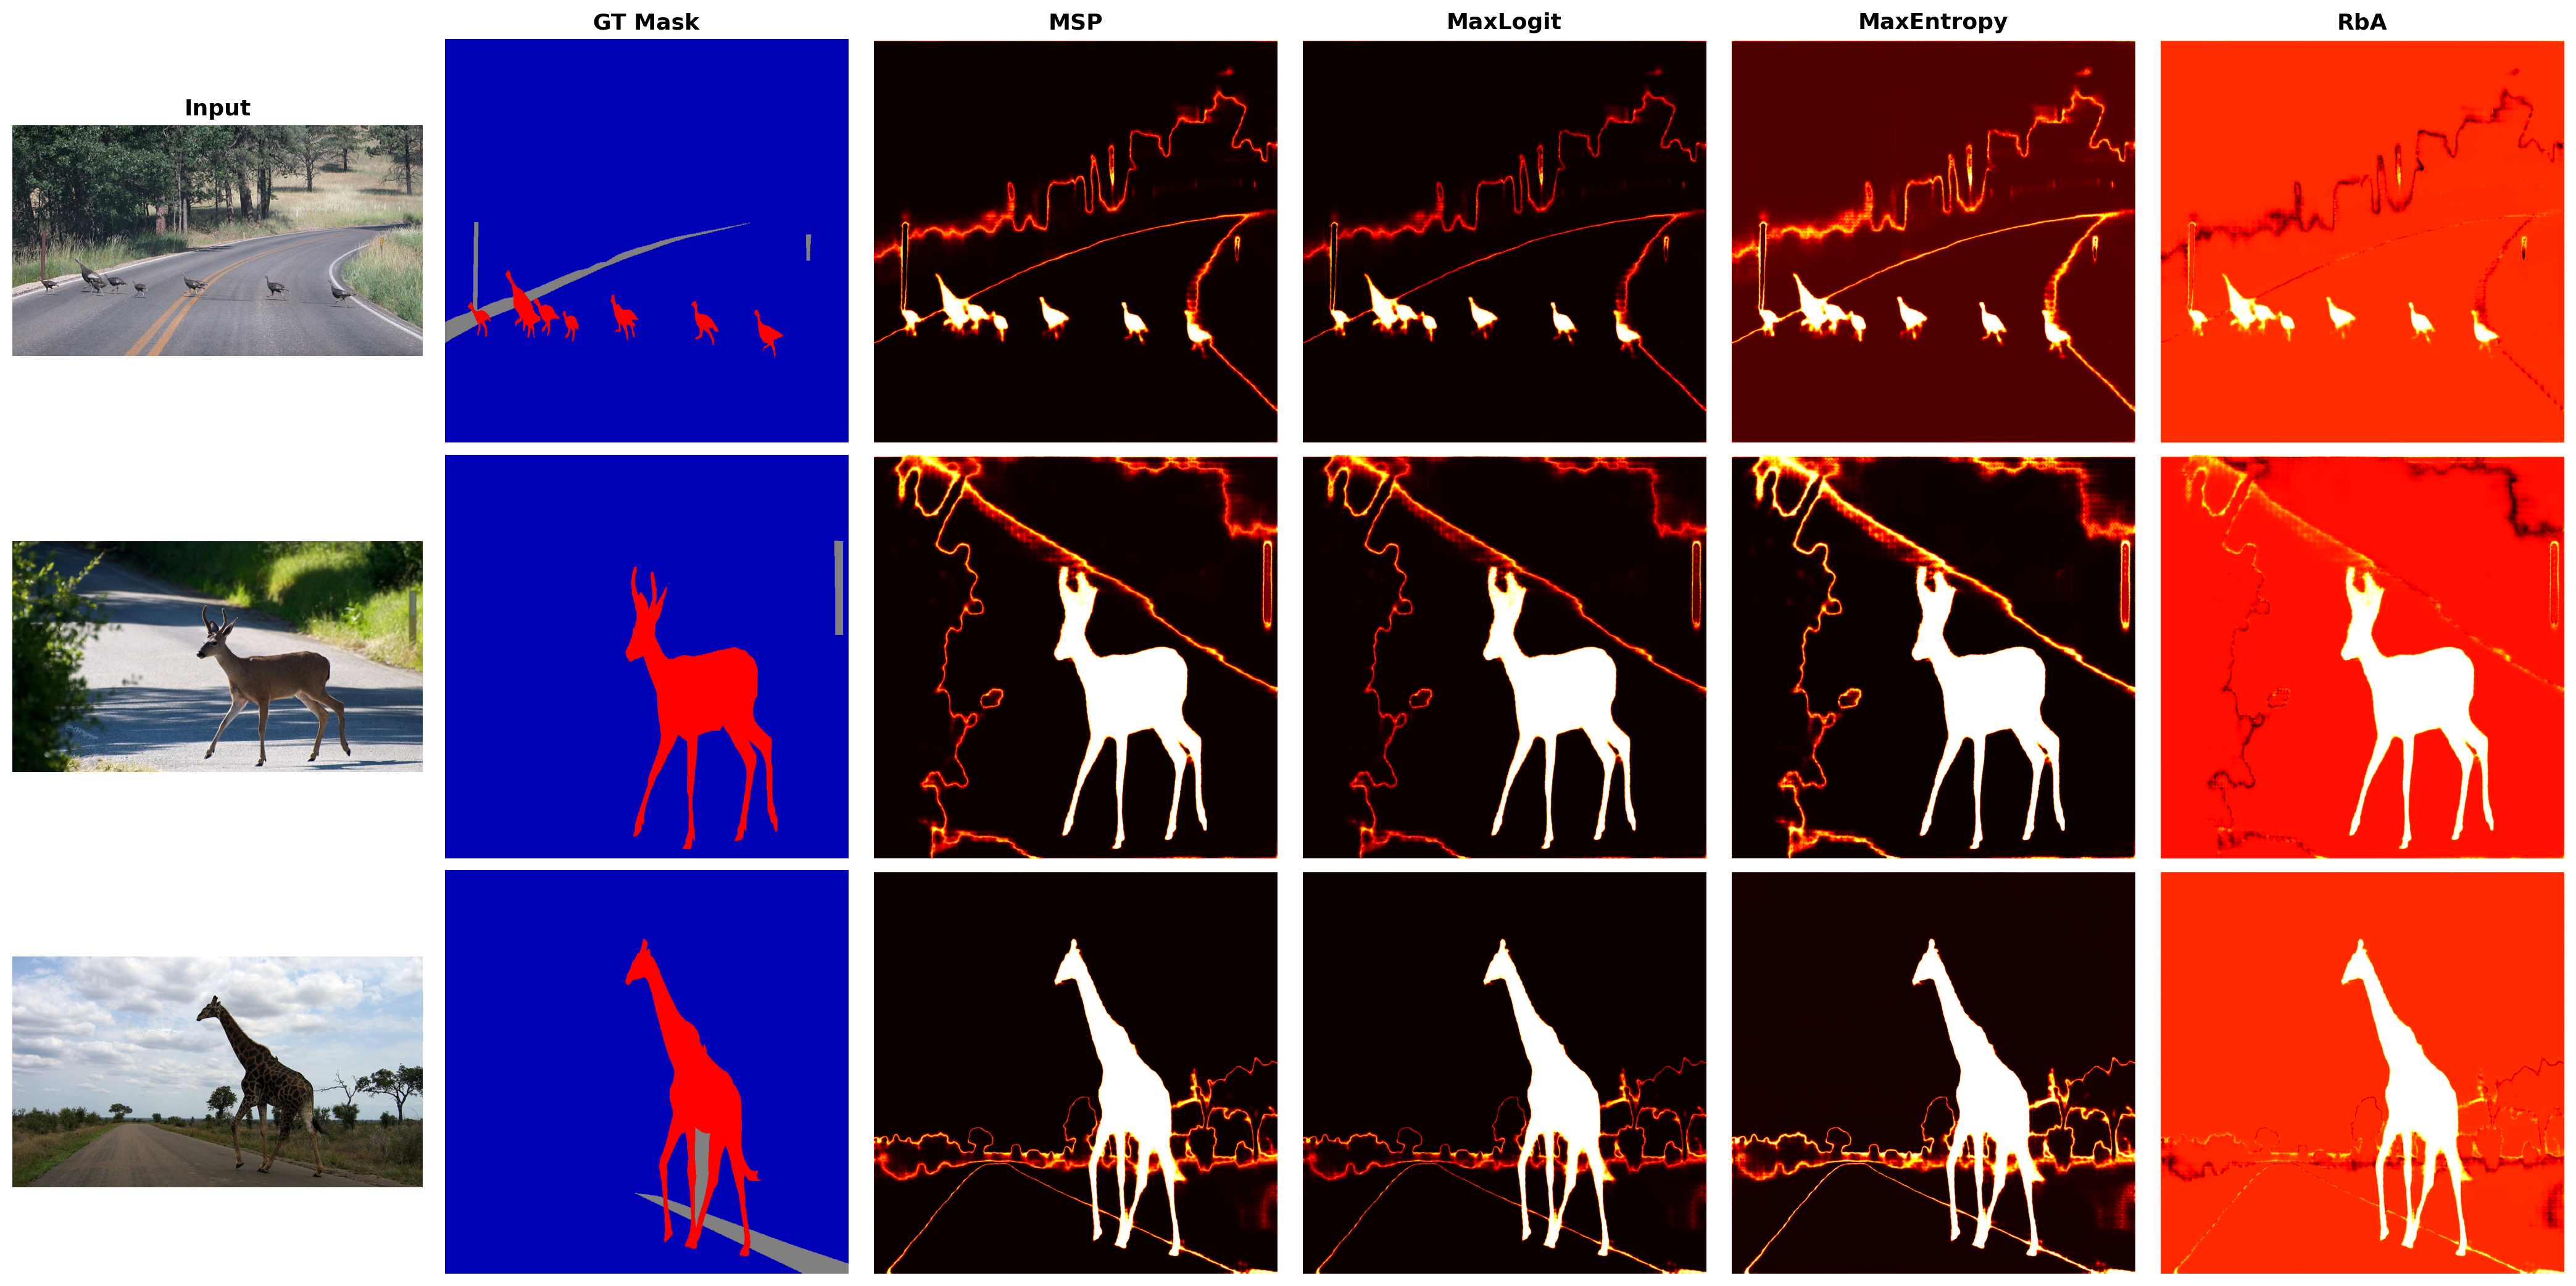
\includegraphics[width=\linewidth]{results/figures/step8/step8_anomaly_maps.png}
\caption{Qualitative comparison of anomaly score maps on RoadAnomaly21. 
Each row shows an input image alongside score maps produced by MSP, MaxLogit, 
MaxEntropy, and RbA for EoMT-Cityscapes.}
\label{fig:step8}
\end{figure}
\paragraph{Comparison of scoring functions.}
Interesting finding here is that MaxLogit beats MSP and MaxEntropy on ERFNet (38.31 vs 29.09 vs 30.96 on RA-21), but on EoMT they are almost same.
This result shows that scoring-method choice depends on the architecture.

\begin{table*}[!tp]
\centering
\caption{Temperature scaling results across the three models. Only $T \in \{0.5, 1.0, 2.0\}$ shown; intermediate values $T \in \{0.75, 1.1, 1.5\}$ follow the same trend. AuPRC ($\uparrow$, \%) and FPR95 ($\downarrow$, \%) on five benchmarks. RbA is omitted for ERFNet as it is incompatible with pixel-based architectures.}
\label{tab:temperature_combined}
\resizebox{\textwidth}{!}{
\begin{tabular}{llc|cc|cc|cc|cc|cc}
\toprule
 & & \multicolumn{2}{c|}{RA-21} & \multicolumn{2}{c|}{RO-21} & \multicolumn{2}{c|}{FS L\&F} & \multicolumn{2}{c|}{FS Static} & \multicolumn{2}{c}{RoadAnom} \\
Model & Method & $T$ & AuPRC$\uparrow$ & FPR95$\downarrow$ & AuPRC$\uparrow$ & FPR95$\downarrow$ & AuPRC$\uparrow$ & FPR95$\downarrow$ & AuPRC$\uparrow$ & FPR95$\downarrow$ & AuPRC$\uparrow$ & FPR95$\downarrow$ \\
\midrule
ERFNet & MSP & 0.5 & 27.05 & 62.75 & 2.42 & 63.24 & 1.28 & 66.73 & 6.6 & 43.48 & 12.19 & 82.04 \\
 &  & 1.0 & 29.09 & 62.57 & 2.71 & 65.27 & 1.75 & 50.62 & 7.47 & 41.84 & 12.42 & 82.59 \\
 &  & 2.0 & 30.6 & 65.05 & 3.0 & 72.74 & 2.69 & 47.92 & 9.54 & 41.29 & 12.64 & 84.58 \\
 & MaxEntropy & 0.5 & 28.58 & 62.74 & 2.64 & 63.73 & 1.59 & 52.82 & 7.04 & 43.2 & 12.33 & 82.26 \\
 &  & 1.0 & 30.96 & 62.67 & 3.04 & 65.95 & 2.58 & 50.19 & 8.84 & 41.55 & 12.67 & 82.76 \\
 &  & 2.0 & 30.27 & 67.09 & 2.97 & 75.98 & 3.51 & 47.1 & 11.72 & 41.75 & 12.79 & 85.6 \\
\midrule
EoMT-Cityscapes & MSP & 0.5 & 74.21 & 33.73 & 90.1 & 0.55 & 25.4 & 14.91 & 54.33 & 34.94 & 75.51 & 19.37 \\
 &  & 1.0 & 74.36 & 33.73 & 90.11 & 0.55 & 25.42 & 14.9 & 54.35 & 34.94 & 75.69 & 19.31 \\
 &  & 2.0 & 74.55 & 33.73 & 90.11 & 0.55 & 25.44 & 14.9 & 54.36 & 34.93 & 75.87 & 19.28 \\
 & MaxEntropy & 0.5 & 77.43 & 33.68 & 90.09 & 0.59 & 29.55 & 14.83 & 53.21 & 34.91 & 78.43 & 19.03 \\
 &  & 1.0 & 77.88 & 33.6 & 90.01 & 0.68 & 29.56 & 14.72 & 52.51 & 34.84 & 78.14 & 18.79 \\
 &  & 2.0 & 77.91 & 33.53 & 89.97 & 0.72 & 29.01 & 14.65 & 51.46 & 34.77 & 77.43 & 18.63 \\
 & RbA & 0.5 & 69.57 & 76.02 & 73.77 & 99.95 & 26.0 & 67.27 & 55.85 & 84.55 & 74.12 & 44.02 \\
 &  & 1.0 & 69.99 & 80.06 & 86.97 & 99.95 & 25.97 & 8.79 & 56.11 & 82.68 & 74.62 & 20.41 \\
 &  & 2.0 & 70.83 & 91.98 & 88.25 & 99.94 & 25.92 & 10.05 & 55.91 & 35.88 & 75.09 & 17.96 \\
\midrule
EoMT-Fine-tuned & MSP & 0.5 & 58.59 & 98.6 & 73.69 & 25.1 & 27.07 & 26.22 & 53.35 & 39.78 & 54.96 & 16.27 \\
 &  & 1.0 & 57.15 & 98.61 & 73.61 & 25.09 & 27.11 & 26.16 & 53.41 & 39.74 & 54.99 & 16.22 \\
 &  & 2.0 & 56.61 & 98.62 & 73.57 & 25.09 & 27.13 & 26.15 & 53.43 & 39.72 & 55.0 & 16.2 \\
 & MaxEntropy & 0.5 & 54.1 & 98.71 & 73.43 & 28.83 & 27.91 & 26.21 & 53.87 & 39.53 & 55.83 & 15.28 \\
 &  & 1.0 & 54.49 & 98.82 & 72.62 & 57.49 & 28.56 & 26.33 & 54.27 & 39.25 & 56.22 & 14.78 \\
 &  & 2.0 & 54.65 & 98.82 & 71.69 & 60.82 & 29.18 & 26.24 & 54.5 & 38.76 & 56.33 & 14.51 \\
 & RbA & 0.5 & 51.52 & 99.53 & 62.1 & 99.98 & 31.42 & 78.97 & 56.29 & 89.51 & 52.39 & 81.57 \\
 &  & 1.0 & 51.82 & 99.85 & 64.22 & 99.98 & 30.61 & 26.92 & 56.29 & 90.34 & 56.14 & 13.38 \\
 &  & 2.0 & 51.88 & 99.87 & 66.12 & 99.98 & 30.36 & 24.49 & 55.73 & 89.65 & 56.57 & 12.09 \\
\bottomrule
\end{tabular}}
\end{table*}

RbA has a different pattern in here. It achieves highest AuPRC on FS L\&F (30.61) and FS Static (56.29) for EoMT-Fine-tuned. 
However, it also produces high score for FPR95, so it separates the outlier but it is too sensitive so it makes a lot of false alarms.  


%\paragraph{Qualitative results.}
%Figure~\ref{fig:step8} shows anomaly score maps for the four scoring methods on representative RoadAnomaly21 images.

\subsection{Temperature Scaling Study}

For temperature scaling, we tried $T \in \{0.5, 0.75, 1.0, 1.1, 1.5, 2.0\}$ on MSP, MaxEntropy, and RbA 
for EoMT-Cityscapes, EoMT-Fine-tuned, and ERFNet.
Main finding that AuPRC is mostly stable across $T$ (Table~\ref{tab:temperature_combined}).
\begin{itemize}
    \item In EoMT-Cityscapes (Table~\ref{tab:temperature_combined}), MSP AuPRC on RA-21 stays in a 0.3\% window, and MaxEntropy stays in a 0.5\% window.
    \item In EoMT-Fine-tuned (Table~\ref{tab:temperature_combined}), It follows similar pattern as EoMT-Cityscapes
    \item In ERFNet (Table~\ref{tab:temperature_combined}), MSP on RA-21 has a change range for 3\%, but its AuPRC is so low that the gain is not meaningful. 
\end{itemize}

Interesting finding that RbA's AuPRC is stable, but its FPR95 swings with T:
\begin{itemize}
    \item EoMT-Cityscapes RbA on FS L\&F: FPR95=67.27 at T=0.5 vs 8.79 at T=1.0
    \item EoMT-Cityscapes RbA on RoadAnomaly: FPR95's score decreases from 20.41 at T=1.0 to 17.96 at T=2.0.
    \item EoMT-Fine-tuned RbA on RoadAnomaly: FPR95 = 81.57 at T=0.5 vs 12.09 at T=2.0
\end{itemize}

As result, we found that T=1.0 is competitive for AuPRC most settings. Temperature scaling doesn't meaningfully improve AuPRC, and can shift the FPR95 results, especially for RbA, but it is not a consistent gain.
Post-hoc temperature calibration is not a reliable method for improving anomaly segmentation on these benchmarks.
\section{Discussion}
\label{sec:discussion}

\paragraph{Mask-based architectures help anomaly detection.}
\todo{Summarize the central empirical finding.}  
% e.g., "Our results show that EoMT consistently outperforms ERFNet on most 
% anomaly benchmarks, supporting the hypothesis that mask classification 
% provides a stronger inductive bias for detecting out-of-distribution regions."

\todo{Explain why, briefly.}  
% e.g., "Because each query in EoMT learns a near-independent one-vs-all 
% classifier, regions claimed by no query produce a clean rejection signal — 
% something a per-pixel softmax model cannot replicate."

\paragraph{Fine-tuning recovers most of the closed-set gap.}
\todo{State the main fine-tuning finding.}  
% "Fine-tuning EoMT-COCO on Cityscapes closes most of the mIoU gap to native 
% training (XX.XX\% vs YY.YY\%) and brings anomaly detection performance to 
% a comparable level, even with a frozen backbone and 20 epochs of training."

\todo{Comment on efficiency.}  
% "This suggests that broad pre-training on COCO transfers efficiently to 
% road scenes, and full backbone updates are not required."

\paragraph{Limitations.}
\todo{Acknowledge limits.}  
% Two or three things: small compute budget (Colab L4, ~20 epochs only); 
% smaller evaluation subsets than the full benchmarks; no outlier-supervised 
% baselines (PEBAL, DenseHybrid) for comparison. RbA has high FPR@95 trade-off.

\paragraph{Future work.}
\todo{One or two directions.}  
% e.g., "Extending fine-tuning to unfrozen backbone training, evaluating 
% on the full benchmark splits, and combining post-hoc scores with light 
% outlier exposure are natural next steps."
\section{Conclusion}
\label{sec:conclusion}

\todo{Recap problem.}  
% "We studied semantic segmentation and anomaly detection for road scenes 
% using the encoder-only mask transformer EoMT, comparing it to the pixel-based 
% baseline ERFNet."

\todo{Recap method.}  
% "We fine-tuned EoMT-COCO on Cityscapes under a frozen-backbone, mixed-precision 
% regime, and evaluated four post-hoc anomaly scoring functions across five 
% benchmarks."

\todo{Recap main finding 1 (semantic seg).}  
% "Fine-tuning recovers most of the closed-set performance gap between a 
% COCO-pretrained model and a model trained natively on Cityscapes."

\todo{Recap main finding 2 (anomaly seg).}  
% "EoMT outperforms ERFNet on most anomaly benchmarks, and RbA — applicable 
% only to mask-based architectures — provides a complementary signal to the 
% softmax-based scoring functions."

\todo{Closing sentence.}  
% "These results suggest that mask classification is a promising direction 
% for safety-critical perception, where detecting out-of-distribution objects 
% matters as much as classifying known ones."
\section*{Acknowledgments}
\label{sec:acknowledgments}

\begin{itemize}
    \item We declare that Generative AI tools were not used for writing the project report
    \item For code development of the project, we used Claude Opus 4.7 and 4.6 by Anthropic. This tool is used for these reasons:
    \begin{itemize}
        \item Debugging errors, catching bugs, fixing memory issues during large-scale evaluation
        \item Understanding the EoMT and ERFNet code structure
        \item Reviewing the formulas, and help with the structuring the repository
        \item Performance optimization, helping to change data-loading patterns that reduced runtime
    \end{itemize}
    All generated code was reviewed, tested, and integrated by the authors. All decisions like 
    model choice, training configuration, evaluation protocol, dataset selection and analysis of experimental
    results were made by the authors.
\end{itemize}

{
    \small
    \bibliographystyle{ieeenat_fullname}
    \bibliography{main}
}

% WARNING: do not forget to delete the supplementary pages from your submission 
% \input{sec/X_suppl}

\end{document}
